% Name: Dyck path
% Description: A Dyck path of length 8, four up steps and four down steps that never dip below the axis, one of the 14 counted by the Catalan number C₄.
% Tags: Dyck path, Catalan numbers, lattice path, combinatorics

\usepackage{amsmath}

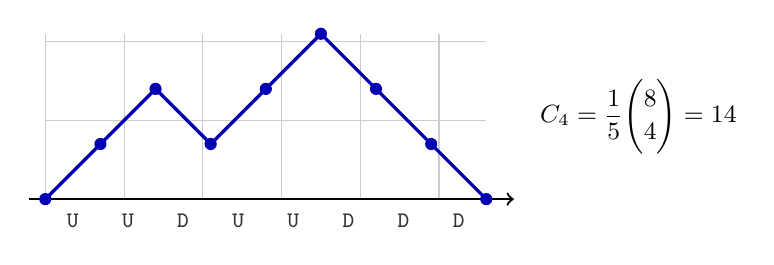
\begin{tikzpicture}[x=7mm, y=7mm, every node/.style={font=\small}]
  \draw[gray!40, thin] (0,0) grid (8,3);
  \draw[thick, ->] (-0.3,0) -- (8.5,0);
  % U U D U U D D D: heights 1, 2, 1, 2, 3, 2, 1, 0
  \draw[very thick, blue!70!black, line join=round] (0,0) -- (1,1) -- (2,2) -- (3,1) -- (4,2) -- (5,3) -- (6,2) -- (7,1) -- (8,0);
  \foreach \x/\y in {0/0, 1/1, 2/2, 3/1, 4/2, 5/3, 6/2, 7/1, 8/0} \fill[blue!70!black] (\x,\y) circle (2.2pt);
  \foreach \s [count=\i from 0] in {U,U,D,U,U,D,D,D} \node[font=\footnotesize\ttfamily, gray!40!black] at (\i+0.5,-0.4) {\s};
  \node[anchor=west] at (8.8,1.5) {$C_4 = \dfrac{1}{5}\dbinom{8}{4} = 14$};
\end{tikzpicture}
